\section{Python Parse Error Analysis}
\label{sec:error-analysis}

\subsection{Parse Errors in Real life}
\label{sec:error-analysis:syntax}

\begin{figure}[h]
  \centering
  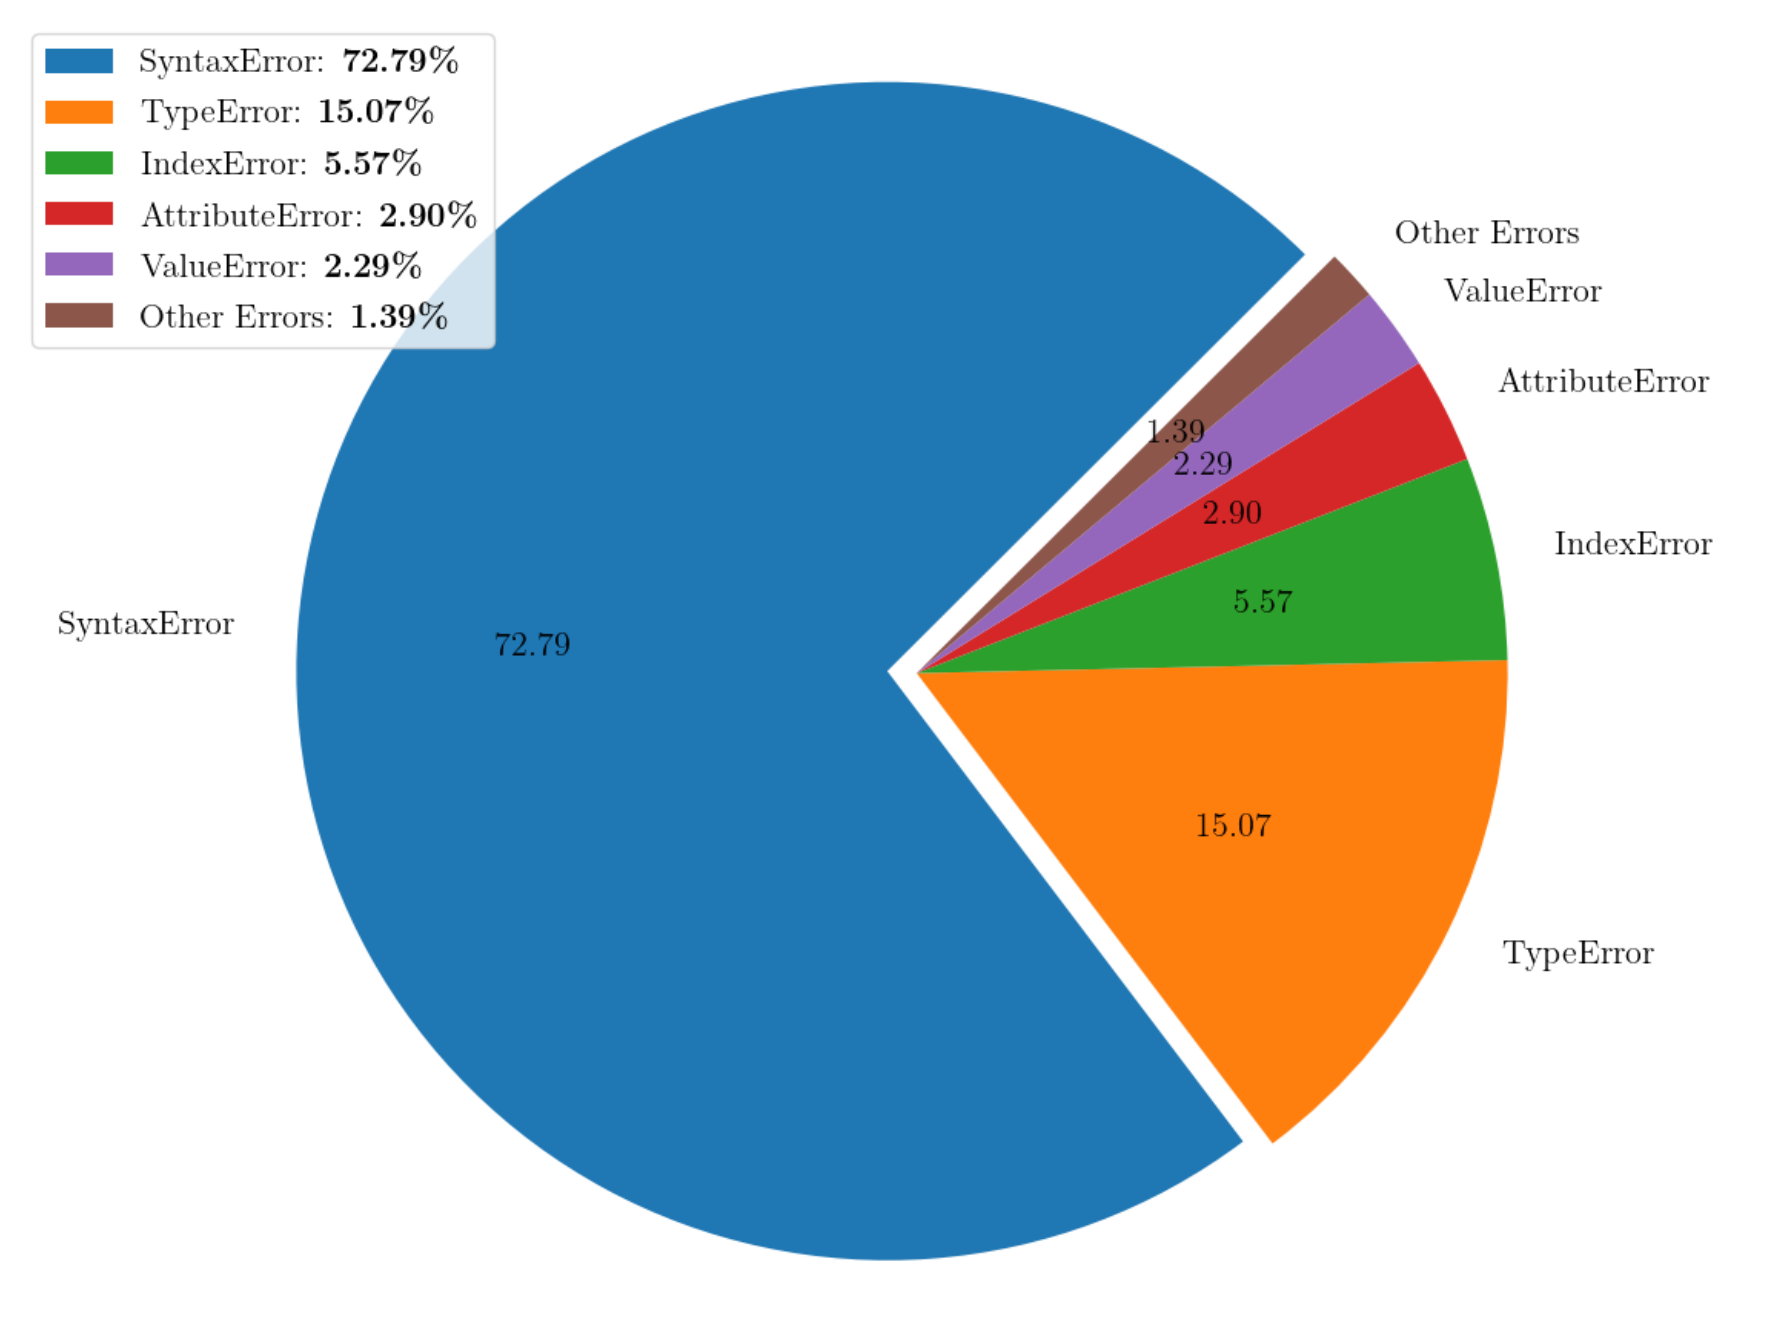
\includegraphics[width=0.8\linewidth]{error-statistics.png}
  \caption{The error type distribution.}
  \label{fig:error-statistics}
\end{figure}

Parse errors (or \emph{Syntax Errors}) are usually easier to locate and be
repaired than other algorithmic or runtime errors most of the times
\citep{Denny_2012}. For example, the \emph{Python parser} will immediately
inform the programmer for missing parenthesis in function argument lists or for
not having the proper indents in a statement block. However, we show here that
programmers (especially novices) mostly deal with these kinds of errors on a
daily basis and still spend a considerable amount of time fixing them.

\mypara{Python Syntax Errors}
We have collected a dataset of more than 800,000 erroneous Python programs along
with their fixes from a web-based Python compiler, where novices programmers
(mostly novices) can submit their code online and execute it. When there is an
error, the failed attempt is recorded and associated with the next successful
run of the same fixed code. This process generates a dataset of program pairs.

By analyzing this data, we observe in \autoref{fig:error-statistics} that $72.79
\% $ of all faulty programs failed with a syntax error. This accounts for the
vast majority of the errors that (novice) programmers face with their programs.
This is a strong indication that these parse errors are very common and require
an automated approach of repairing.

\begin{figure}[h]
  \centering
  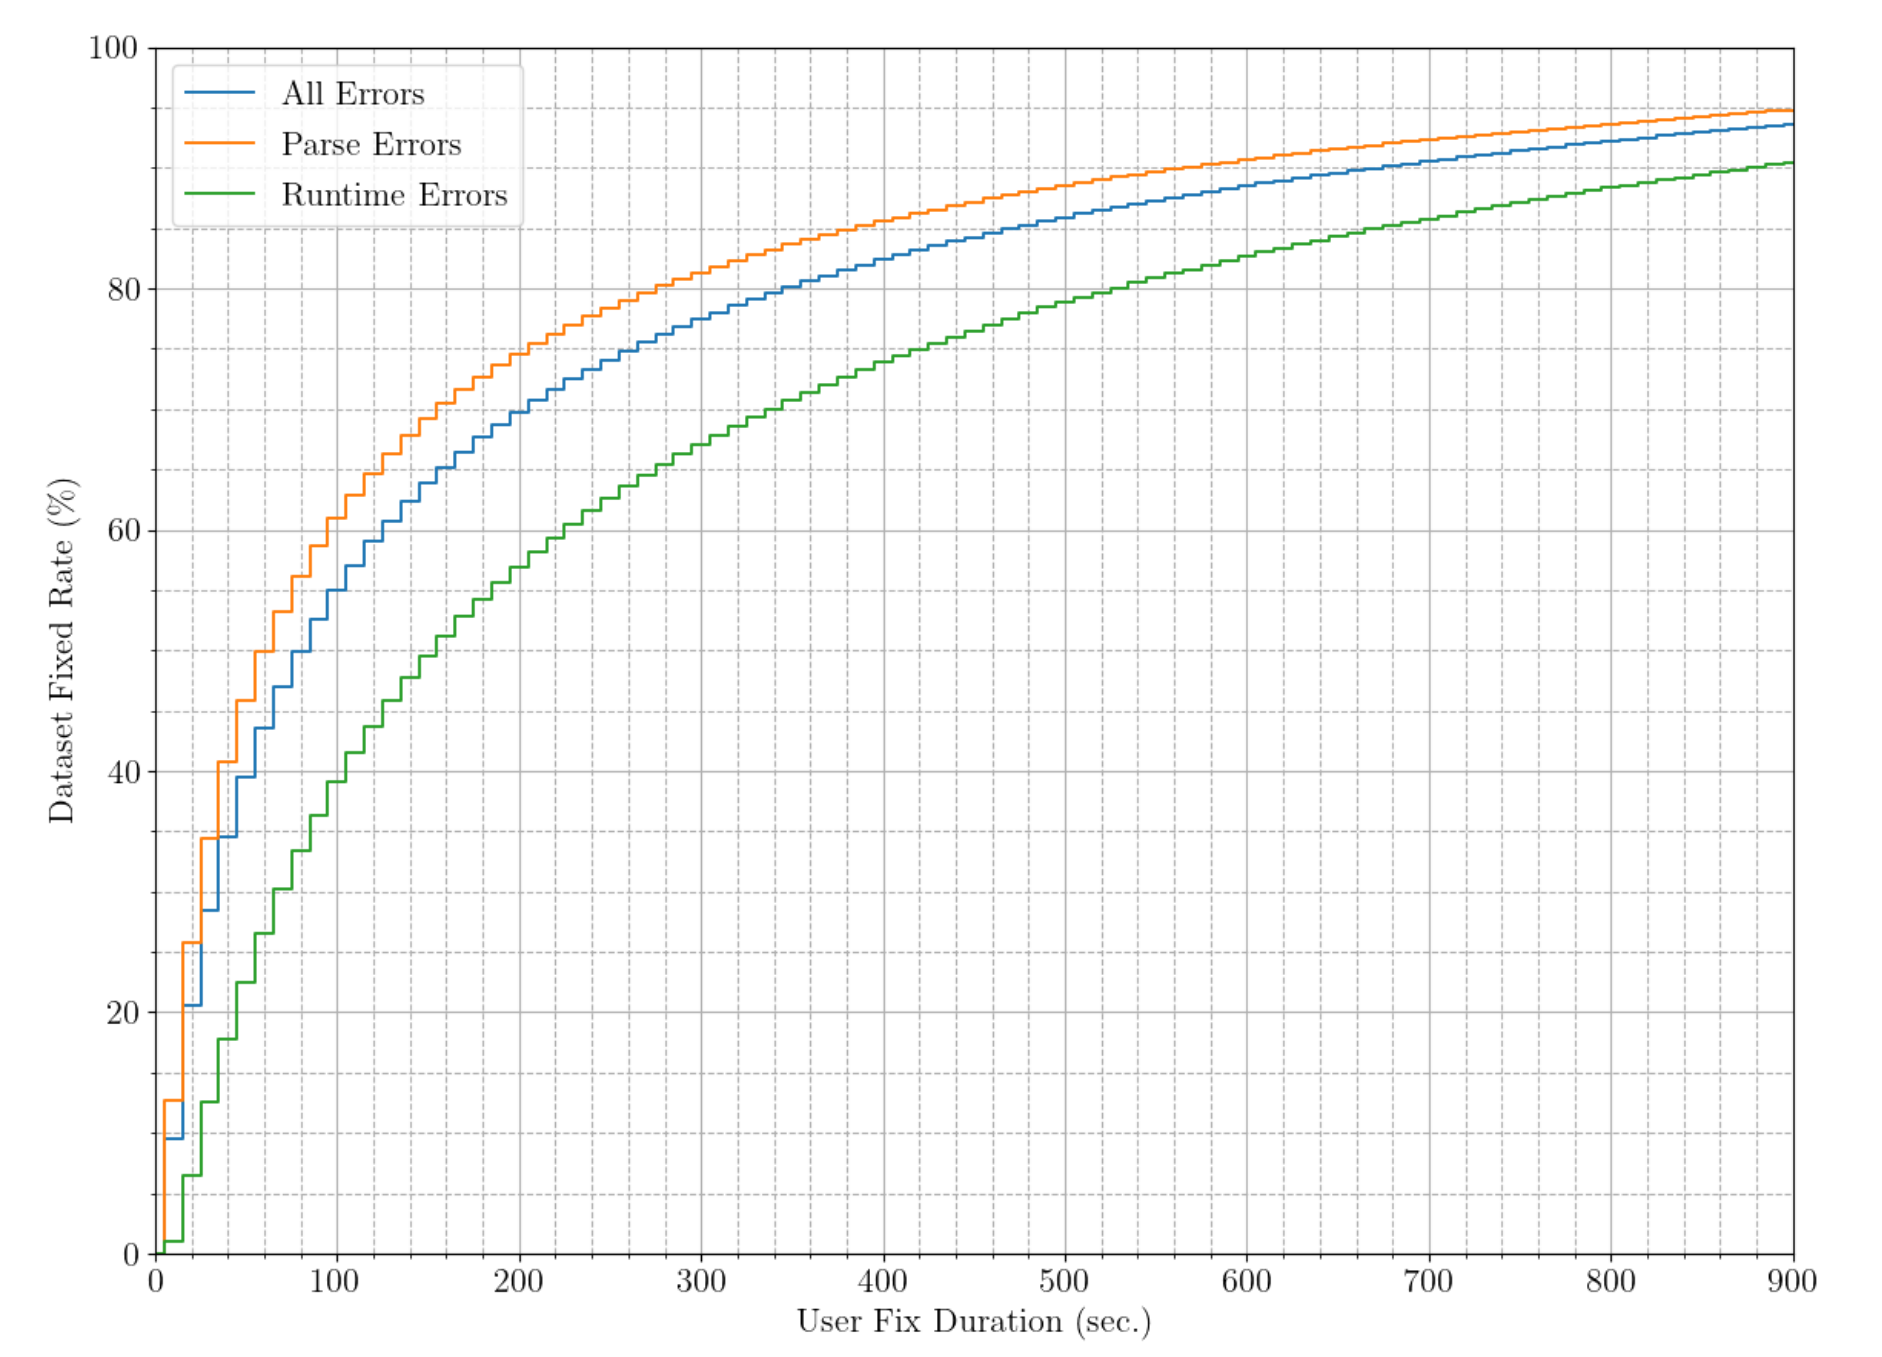
\includegraphics[width=0.9\linewidth]{repair-rate-all-parse.png}
  \caption{The repair rate of the Python dataset for all, syntax and runtime
  errors.}
  \label{fig:repair-rate}
\end{figure}

\mypara{Python repair rate} The web-based compiler that we used to generate our
dataset, also provides us with a \emph{server timestamp}. The timestamp is
associated with each program attempt submission, erroneous or not. The
\emph{repair time} of an erroneous program is calculated by taking the
difference of the two timestamps of the erroneous and fixed program. Although
this method is not the most accurate, it can still be viewed as an appropriate
metric of the amount of time it took the programmer to repair the errors in
their program when we have such a large dataset.

We plot in \autoref{fig:repair-rate} the \emph{programmer repair rate}, \ie the
dataset percentage that is repaired under a given amount of time. We include the
repair rate for all the errors, the parse/syntax errors and the rest of the
errors mentioned here as \emph{runtime} errors. As expected, the parse errors
are fixed faster than all the other ones, but not by a large difference. We
observe for example that within 2 minutes, usually $42 \%$ of the runtime
errors, \ie all the errors that do not include the syntax errors, are repaired
and around $65 \%$ of the syntax error. Although, this is a considerable
difference, we observe that there is still a large number of the "simpler" parse
errors that required more than 2 minutes to be fixed. We also observe that only
$50 \%$ of the parse errors are fixed under 1 minute. Therefore, an automated
tool that repairs or parses those programs in a few seconds could be beneficial
for a lot of programmers, novices or not.

\begin{figure}[h]
  \centering
  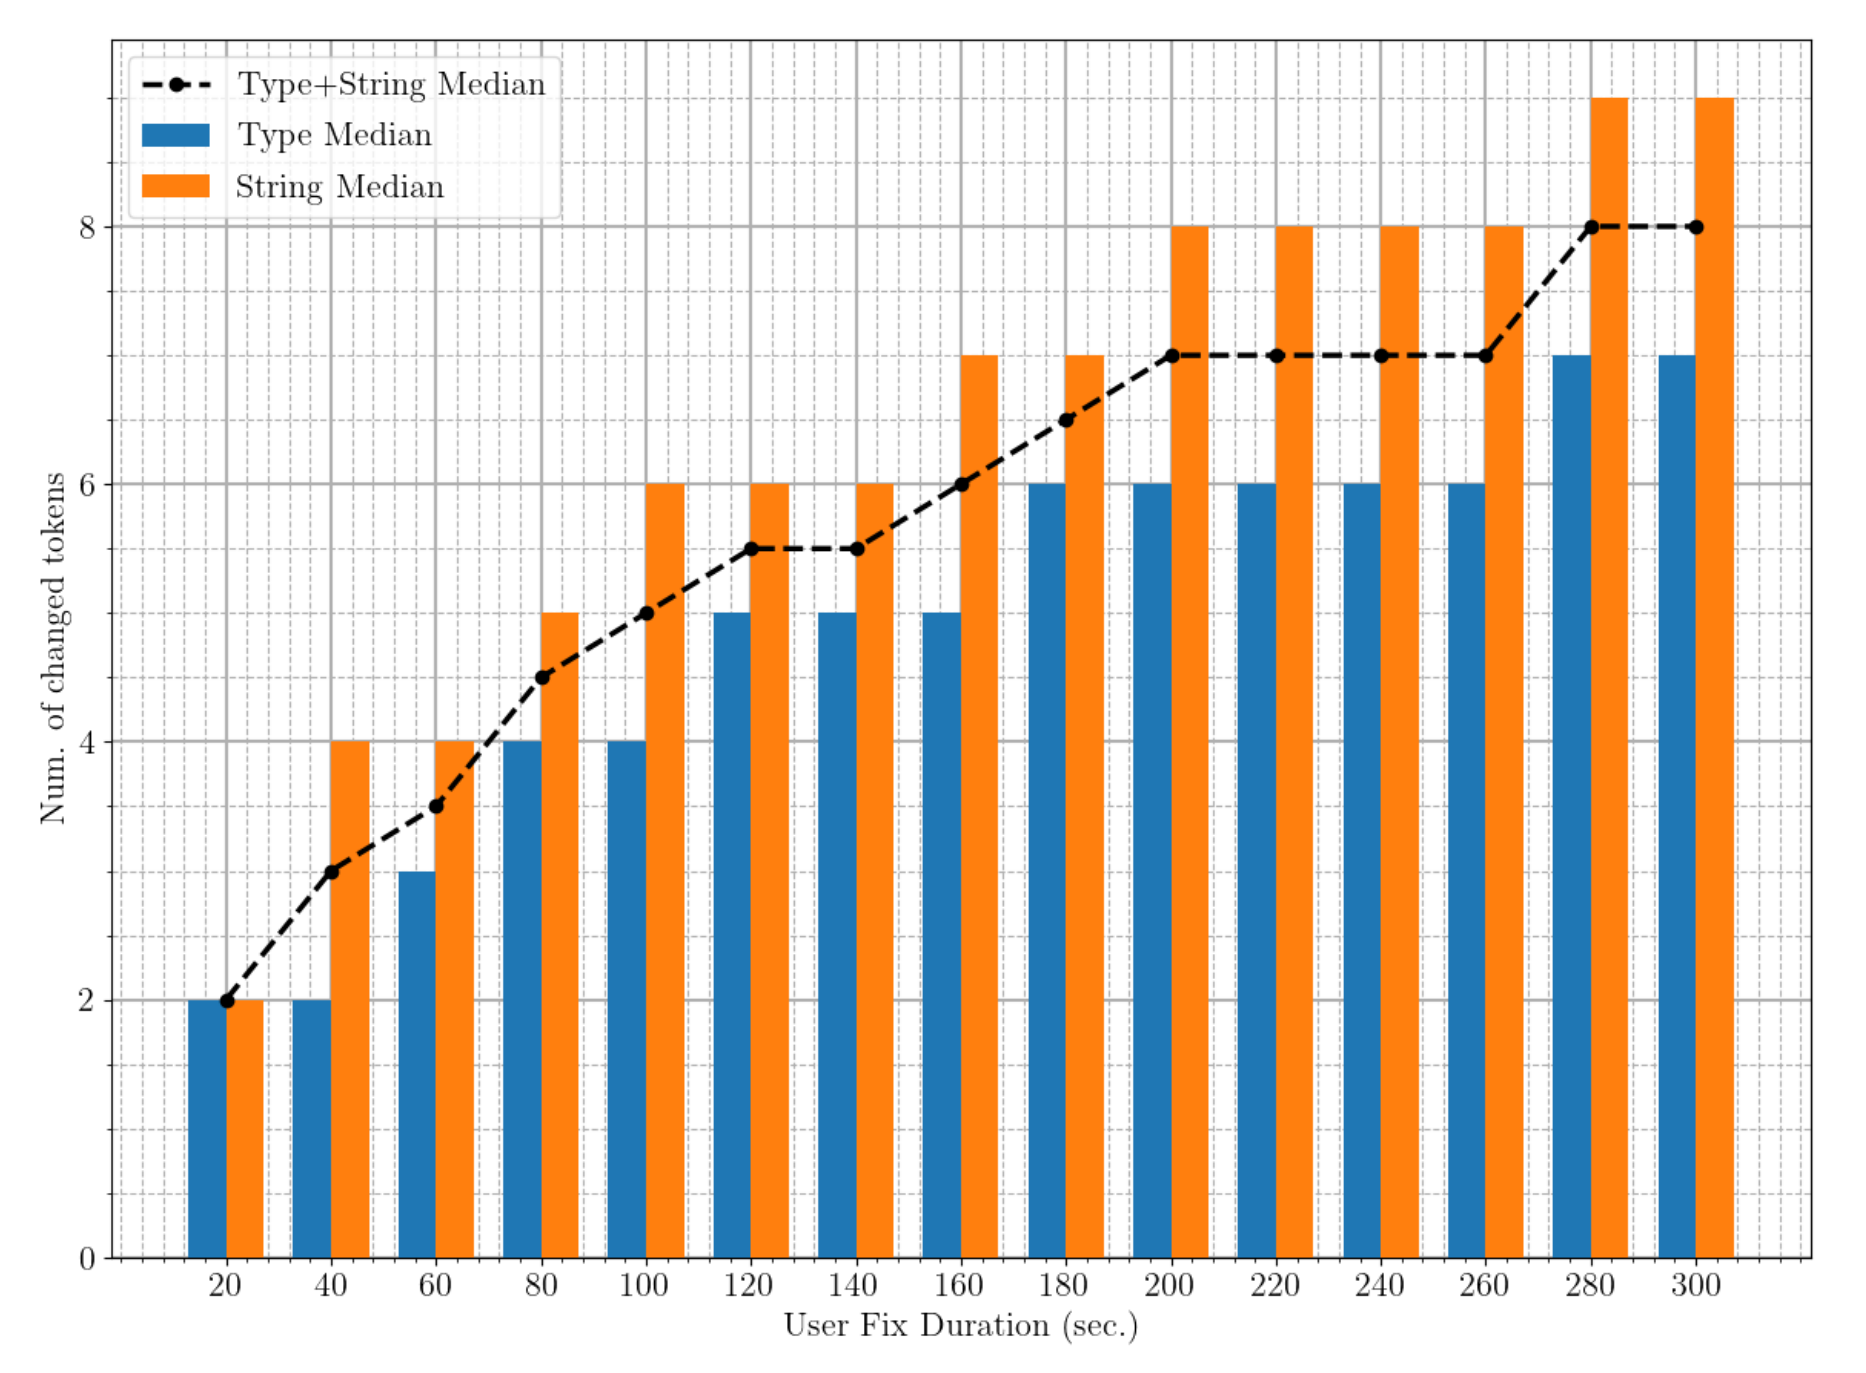
\includegraphics[width=0.9\linewidth]{token-changes.png}
  \caption{The average number of token changes between the erroneous and fixed
  program under the time the user needed to fix the program.}
  \label{fig:token-changes}
\end{figure}

\mypara{Token-level changes} \autoref{fig:token-changes} shows how many token
changes are required to get the parse errors fixed in a given program on average
under that time. As expected, with an increasing number of changes needed at
program to fix all parse errors, more time is needed for the programmers to make
those changes. Additionally, the median token-level changes needed in the lexed
programs (\eg \emph{type diff}) to fix a runtime error is 24 token changes on
average (median is 8), while in order to fix a program with parse errors it
requires 10 token changes on average (median is 3). This results further
indicates that, while simple parse errors can easily and quickly be fixed by the
programmers and the Python parser messages can be enough, they still struggle
fixing programs that have more parse errors that maybe the error message doesn't
even point to.
